\documentclass{article}
\usepackage[T1]{fontenc}
\usepackage[utf8]{inputenc}
\usepackage{geometry}
\usepackage{graphicx}
\usepackage{url,hyperref}
\usepackage{xcolor,listings}
\usepackage{textcomp}
\usepackage{float}
\usepackage[bottom]{footmisc}
\usepackage{fancyvrb}
\usepackage{textcomp}
\usepackage{color}
\usepackage{footnote}
\usepackage{tabularx}
\usepackage[detect-all]{siunitx}
\sisetup{range-phrase = \text{--}}

\usepackage{adjustbox}
\usepackage{multirow}

\makesavenoteenv{table}

\hypersetup{
	colorlinks = true,
	citecolor = green,
	urlcolor = cyan
}

\definecolor{codegreen}{rgb}{0,0.6,0}
\definecolor{codegray}{rgb}{0.5,0.5,0.5}
\definecolor{codepurple}{HTML}{C42043}
\definecolor{backcolour}{HTML}{F2F2F2}
\definecolor{bookColor}{cmyk}{0,0,0,0.90}
\color{bookColor}

\lstset{upquote=true}

\lstdefinestyle{mystyle}{
	backgroundcolor=\color{backcolour},
	commentstyle=\color{codegreen},
	keywordstyle=\color{codepurple},
	numberstyle=\numberstyle,
	stringstyle=\color{codepurple},
	basicstyle=\footnotesize\ttfamily,
	breakatwhitespace=false,
	breaklines=true,
	captionpos=b,
	keepspaces=true,
	numbers=left,
	numbersep=10pt,
	showspaces=false,
	showstringspaces=false,
	showtabs=false,
}

\title{
	Web Information Extraction and Retrieval\\
	Programming Assignment 3: \\
	Document indexing and querying
}
\author{
	Marko Prelevikj\\
	63130345\\
	\texttt{mp2638@student.uni-lj.si}
	\and
	Gojko Hajduković\\
	63180431\\
	\texttt{gh8590@student.uni-lj.si}
	\and
	Stefan Ivanišević\\
	63170405\\
	\texttt{si0539@student.uni-lj.si}
}
\date{May 2019}

\begin{document}
	
	\maketitle
	\section{Introduction}
	With the increasing development of information technologies, in the modern, digital era, most of the documents and information are stored in a digital format in order to be easy accessible to everyone within the globe. Many of the problems arose when the increasing amount of data needed to be stored efficiently in order for users to have quick access to the information they needed. In many information systems where some type of search is required, first natural approach in finding related words, queries within the documents was the naive approach of sequentially looking into all of the documents for specific words, which was very inefficient regarding time and space. Nowadays, the most widely used and efficient way of storing the data in order to be searched from quickly is the concept of \textit{Inverted Index}.
	
	\textit{Inverted index} represents an efficient technique for storing mappings of words, content to its locations in a single or a set of documents. In this paper we introduce our implementation of an Inverted Index. Firstly, we preprocess the documents, then build an inverted index from the preprocessed content, and then allow the users to quickly search for the content they need by a simple \href{https://en.wikipedia.org/wiki/Read%E2%80%93eval%E2%80%93print_loop}{ REPL} interface. We also implemented a not-so-naive approach for \textit{sequential file reading} in order to compare the efficiency of the inverted index.
	
	\section{Data Pre-processing} \label{sec:Preprocess}
	For a more efficient indexing step, we need to preprocess the corpus. The corpus contains 1416 crawled web pages. Each web page is processed in the same manner as described in continuation.
	
	First, we extract the text data using the package \href{https://pypi.org/project/inscriptis/}{inscriptis} and unify the text into lowercase. Due to the poor performance of the dependent library which leaves behind some \textit{HTML} tags among the content, we extracted them out with regex.
	
	The next step of preprocessing the corpus is content tokenization, i.e. splitting up a textual data into, not necessarily meaningful, words. We have performed it using the \href{https://www.nltk.org/}{nltk.tokenize} package. In order to minimize space complexity of our approach we removed all duplicates occurrences of the tokens. To keep the tokens meaningful, we also removed all tokens belonging to a predefined set of stopwords, and eliminated most of the special characters.
	
	To keep the data retrieval process as efficient as possible, we also tokenized the content of each document without removing the stopwords and special characters. The output of the pre-processing is a dictionary data structure which contains $1416$ keys denoting the source file names. The structure of our pre-processed corpus is available in the listing below. We store this structure on the disk in order to efficiently build the indices and speed-up the sequential data retrieval.
	
	\begin{verbatim}
	{
	"<inputFileName1>": {
	"tokens": ["<token1>", "<token2>", ... , "<tokenN>"],
	"content": ["<word1>", "<word2>", ... , "<wordN>"]
	},
	"<inputFileName2>": {
	"tokens": ["<token1>", "<token2>", ... , "<tokenN>"],
	"content": ["<word1>", "<word2>", ... , "<wordN>"]
	},
	...,
	"<inputFileNameN>": {
	"tokens": ["<token1>", "<token2>", ... , "<tokenN>"],
	"content": ["<word1>", "<word2>", ... , "<wordN>"]
	}
	}
	\end{verbatim}
	
	\section{Index building}
	To be able to benchmark the performance of the indices, we built two different indices: \textit{Inverted Index} and \textit{Sequential Index}. 
	We use the cached pre-processing output in order to efficiently build the indices. In the following subsections we describe how we build the indices.
	
	\subsection{Inverted Index}
	In our implementation of the \textit{Inverted index}, we used a database in order to simulate the inverted index structure. The database structure is consisted of three tables:
	\begin{description}
		\item[\texttt{IndexWord}] consists of all the words indexed from the documents in the corpus, i.e. our dictionary, $D$.
		\item[\texttt{Posting}] consists of a word from \textit{IndexWord}, a document name in which the specific it appears, the frequency of its appearance within the document, and the indices where the word appears in the source document.
		\item[\texttt{Existing}] consists of a column \texttt{doesExist} which we have added in order to indicate whether the inverted index has already been built, as the rebuilding operation is rather costly.
	\end{description}
	
	In order to construct the \textit{Inverted Index} out of the pre-processed corpus, we have constructed a dictionary data structure which is an in-memory replica of the database. With this structure we are able to store all the required information for a given word: the word it appears in, its frequency within the document, and indices where the word appears within the source document.
	
	The next step of our implementation is to store the constructed \textit{Inverted index} in the database. First, we store the list of keys from the \textit{Inverted Index} dictionary in the table \texttt{IndexWord}. The keys represent the set of all unique words from the provided corpus. Then we construct a list which holds all postings in the format \newline \texttt{$[(\mbox{word, documentName, frequency, indexes})]$}.
	
	\subsection{Sequential index}
	
	The \textit{Sequential Index} does not require a special procedure of preparing in order to perform the search. We simply use the pre-processed data to perform the search on.
	
	\section{Data retrieval}
	The data retrieval process (search) is performed on a user provided query which is first pre-processed, to get it in the same form as the rest of the corpus, i.e. it is tokenized. Afterward we are performing the search based on which index has been chosen by the user (either sequential or inverted). Both methods return the results in the same format: a list of tuples containing the cumulative \textit{frequency} per document, the \textit{document} name, and the aggregated \textit{indices} of all results.
	
	\subsection{Inverted Index}
	Search the \textit{Inverted Index} is performed with a single query on the database. The query is shown in Listing~\ref{lst:query}, and it is an excerpt of the \textit{Python} code which is performing the query.
	
	\begin{lstlisting}[  language=SQL,
									label={{lst:query2}},
									deletekeywords={IDENTITY},
									deletekeywords={[2]INT},
									morekeywords={clustered},
									framesep=5pt,
									xleftmargin=0pt,
									framexleftmargin=0pt,,
									frame=tb,
									framerule=0pt ]
	SELECT documentName, sum(frequency) as freq, group_concat(indexes)
	FROM Posting
	-- the following part is filled by Python based on
	-- the length of the tokenized query
	WHERE word IN ({','.join(['?']*len(query))})
	GROUP BY documentName
	ORDER BY freq DESC
	\end{lstlisting}
	
	The query groups together the postings which match the words in the tokenized query, sums up the frequencies from the corresponding files, and aggregates the indices from the source document. The end result is a list of tuples, as previously described.
	
	\subsection{Sequential Index}
	The search for the \textit{Sequential Index} is really simple: We get the pre-processed corpus and we iterate throughout the tokenized file content to get all the matches per file, and keep the track of the matches.
	
	\section{Implementation details}
	Some further implementation details worth noting:
	\begin{description}
		\item[Output printing] Each row from the obtained result is printed in a table as provided in the \href{http://zitnik.si/teaching/wier/PA3.html}{instructions}. The printing is provided by \href{https://pypi.org/project/texttable/}{texttable}.
		
		\item[Snippets] The snippets mark the queried word with \texttt{*} symbols, and include up to 3 words to the left and to the right of the result.
		
		\item[REPL mode] It is possible to enter in an interactive mode where the user is able to: \textit{query} both types of indices, \textit{change} the type of index being queried, force a \textit{recreation} of the index and change the \textit{number of results} printed in the table.
	\end{description}
	
	\section{Query Results}
	This section introduces results of six different queries consisted of up to five words. We obtained identical results by querying both the inverted index and by performing a sequential search in the entire corpus of each word from the given query. The results from the three predefined queries are given in Table~\ref{tab:2}.
	
	Querying the inverted index database is $\approx40$ times faster than sequentially searching through the corpus. We concluded this by implementing a benchmarking function which generates $10$ queries consisted of \numrange{1}{5} randomly selected words from the corpus (each word is independently selected), and executes the search $N$ times. We provide the results in Table~\ref{tab:1}. This test also shows us that the more times we query the index sequentially, the faster we obtain the results. This is as a consequence of an internal caching of the results within python. Another factor is the amount of words the query is consisted of and how many times it appears within the corpus. We present three additional query results in Table~\ref{tab:3}, Table~\ref{tab:4} and Table~\ref{tab:5}, respectively.
	
	\begin{table}[hbt!]
		\centering
		\begin{tabular}{c|c|c}
			\texttt{\# iterations \footnote{Number of iterations performed on each of the 10 randomly generated queries.}}& \texttt{Inverted index} & \texttt{Sequential index}  \\ \hline
			50 & 1.71ms  & 68.34 ms \\
			100 & 1.34 ms & 61.63 ms \\
			250 & 1.15 ms & 56.43 ms \\
			500 & 1.58 ms & 55.47 ms \\
			1000 & 1.19 ms & 56.73 ms
		\end{tabular}
		\caption{Benchmark test on 10 random queries against and \#iterations of both the inverted and sequential index.}
		\label{tab:1}
	\end{table}
	
	\begin{table}[!hbt]
		\begin{adjustbox}{width=1\textwidth}
			\small
			\centering
			\begin{tabularx}{\textwidth}{c|c|c|c|X}
				\texttt{Query}&\texttt{Rank} & \texttt{Frequency} & \texttt{Document} & \texttt{Snippet}  \\ \hline
				\multirow[b]{2}*{\texttt{predelavne  dejavnosti}}& 1& 75 & evem.gov.si.377 & defektolog v zdravstveni *dejavnosti* + dekan ozirom.. dietetik v zdravstveni *dejavnosti* + dimnikar + ... \\ \cline{2-5}
				& 2& 40 & podatki.gov.si.340 & nosilec dopolnilne *dejavnosti* na kmetiji bregar ... šport center interesnih *dejavnosti* ptuj center judovske ... šolskih in obšolskih *dejavnosti* center urbane kulture ... \\ \cline{2-5}
				& 3 & 36 & evem.gov.si.452 & evem›dejavnosti›druge storitvene *dejavnosti* , drugje nerazvrščene ... )druge storitvene  *dejavnosti* , drugje nerazvrščene ... skd šifra zajema *dejavnosti* in storitve , ... začetek in opravljanje *dejavnosti* .predpisi in... \\ \hline
				
				\multirow{3}{*}{\texttt{trgovina}}             &1& 95 & evem.gov.si.651 & govedoreja + druga *trgovina* na drobno v ... prodajalnah + druga *trgovina* na drobno v ...prodajalnah + druga *trgovina* na drobno v ... živili + druga *trgovina* na drobno zunaj ...  \\ \cline{2-5}
				&2& 92 & evem.gov.si.21 & moj e-vem evem›področja *trgovina* tu boste našli ... dejavnosti * druga *trgovina* na drobno v ... prodajalnah * druga *trgovina* na drobno zunaj ... ) * nespecializirana *trgovina* na debelo * ...\\ \cline{2-5}
				&3 & 82 & podatki.gov.si.340 & a dent , *trgovina* in storitve , ... . adria investicije *trgovina* , posredništvo , ... d.o.o . ahatservis *trgovina* in storitve , ... d.o.o . alba *trgovina* in proizvodnja , ... \\ \hline
				
				\multirow{3}{*}{\texttt{social services}} & 1& 5 & e-uprava.gov.si.45 & , retirement * *social* services , health ... retirement * social *services* , health , ...          relationship etc. ? *social* services , health ... etc. ? social *services* , health , ... i obtain financial *social* assistance ? how ...  \\ \cline{2-5}
				&2& 5 & e-uprava.gov.si.5 & , retirement * *social* services , health ... retirement * social *services* , health , ... relationship etc. ? *social* services , health ... etc. ? social *services* , health , ... i obtain financial *social* assistance ? how ... \\ \cline{2-5}
				&3 & 1 & evem.gov.si.661 & records and related *services* ( ajpes) ...  
				
			\end{tabularx}
		\end{adjustbox}
		\caption{Results for pre-defined queries}
		\label{tab:2}
	\end{table}
	
	\begin{table}[!hbt]
		\centering
		\begin{tabularx}{\textwidth}{c|c|c|X}
			\texttt{Rank} & \texttt{Frequency} & \texttt{Document} & \texttt{Snippet}  \\ \hline
			1& 62 & evem.gov.si.661 & english welcome to *the* e-trr system ! ... ) account for *the* payment of the ... the payment of *the* initial capital of ... a precondition for *the* establishing of a ... a company in *the* register of companies ...  \\ \hline
			2& 51 & podatki.gov.si.490 & povezava header - *middle* left navigation * ... + kmetijstvo , *ribištvo* , gozdarstvo in ... , ribištvo , *gozdarstvo* in prehrana + ... portalu header - *middle* right navigation * ... povezave header - *middle* left navigation * ...  \\ \hline
			3 & 49 & podatki.gov.si.239 & r povezava header - *middle* left navigation * ... + kmetijstvo , *ribištvo* , gozdarstvo in ... ,ribištvo , *gozdarstvo* in prehrana + ... portalu header - *middle* right navigation * ... povezave  header - *middle* left navigation * ...
		\end{tabularx}
		\caption{Results of the query "the middle gozdarstvo kontakt ribšitvo"}
		\label{tab:3}
	\end{table}
	
	\begin{table}[!hbt]
		\centering
		\begin{tabularx}{\textwidth}{c|c|c|X}
			\texttt{Rank} & \texttt{Frequency} & \texttt{Document} & \texttt{Snippet}  \\ \hline
			1& 10 & podatki.gov.si.494&  državni organi energetika *cene* električne energije za ... z naslovom `` *cene* električne ... nadaljujte ... državni organi energetika *cene* energentov , slovenija ... z naslovom `` *cene* energentov , ... ... državni organi energetika *cene* za zemeljski plin ... \\ \hline
			2& 6 & podatki.gov.si.506 & državni organi energetika *cene* za zemeljski plin ... z naslovom `` *cene* za zemeljski plin ... državni organi energetika *cene* za zemeljski plin ... z naslovom `` *cene* za zemeljski plin ... državni organi energetika *cene* električne energije za ... \\ \hline
			3 & 6 & podatki.gov.si.508 & državni organi energetika *cene* električne energije za ... z naslovom `` *cene* električne ... nadaljujte ... državni organi energetika *cene* za zemeljski plin ... z naslovom `` *cene* za zemeljski plin ... državni organi energetika *cene* za zemeljski plin ...
		\end{tabularx}
		\caption{Results of the query "cene 2018"}
		\label{tab:4}
	\end{table}

	\begin{table}[!hbt]
		\centering
		\begin{tabularx}{\textwidth}{c|c|c|X}
			\texttt{Rank} & \texttt{Frequency} & \texttt{Document} & \texttt{Snippet}  \\ \hline
			1& 13 & evem.gov.si.227& pogoji : * *zakon* o sodiščih in ... in če drug *zakon* ali uredba določa ... za pravosodje * *zakon* o državnem tožilstvu ... jih določa ta *zakon* , ter opravlja ... za pravosodje * *zakon* o alternativnem reševanju ...  \\ \hline
			2& 11 & evem.gov.si.224 & pogoji : * *zakon* o varstvu okolja ... in prostor * *zakon* o zasebnem varovanju ... veljavno licenco . *zakon* o zasebnem varovanju ... za obrambo * *zakon* o varnosti v ... za infrastrukturo * *zakon* o varstvu pred ... \\ \hline
			3 & 9 & e-prostor.gov.si.13 &'' . * *zakon* o evidentiranju nepremičnin ... ) . * *zakon* o nadzoru države ... 35/2010 ) ta *zakon* določa organizacijo in ... v 10. členu *zakon* določa , da ... v 12. členu *zakon* določa pristojnost geodetske ...                                                        
		\end{tabularx}
		\caption{Results of the query "naslovni zakon"}
		\label{tab:5}
	\end{table}
	
	\section{Analysis} \label{sec:analysis}
	
	The inverted index has a total of $29667$ words, and $1416$ documents. 
	We summed up the basic statistics of the documents in Table~\ref{tab:1}. Based on the statistics shown in Table~\ref{tab:1} we can conclude that we most retrieved the most tokens from the document named \texttt{podatki.gov.si.340.html}, which consequently leads to having the most occurrences which ranks it as the biggest document.
	
	We summed up the basic statistics of the words occurring in our provided corpus in Table~\ref{tab:2}. We also calculated a weighted mean frequency of the words from the corpus with the formula presented in Equation~\ref{eq:1}.
	\begin{equation}\label{eq:1}
	f_{wi} = \frac{\scriptstyle \sum_{d \in D} f_{i,d}}{\scriptstyle \sum_{d \in D} f_d} * \frac{\scriptstyle \sum_{d \in D} occurence_d(i)}{|D|}
	\end{equation}
	where $f_{wi}$ denotes the weighted frequency of the $i^{th}$ word, $f_{i,d}$ denotes the frequency of the $i^{th}$ word in the $d^{th}$ document, $n_d$ denotes the sum of frequencies of all words appearing in the $d^{th}$ word. The function $occurence_d(i)$ is calculated as presented in Equation~\ref{eq:2}. $D$ denotes the set of documents, i.e. the corpus, whereas $|D|$ denotes the number of documents in the corpus. Translated into \textit{SQL}, we used the query in the listing below.
	
	\begin{equation} \label{eq:2}
	occurrence_d(i)= \left\{
	\begin{array}{ll}
	1 & i \in d \\
	0 & i \not\in d\\
	\end{array} 
	\right. 
	\end{equation}
	
	\begin{lstlisting}[ language=SQL,
									label={{lst:query2}},
									deletekeywords={IDENTITY},
									deletekeywords={[2]INT},
									morekeywords={clustered},
									framesep=5pt,
									xleftmargin=0pt,
									framexleftmargin=0pt,
									frame=tb,
									framerule=0pt ]
	SELECT word, avg(frequency) * sum(1)/1416.0 weightedFreq, sum(1) occurence
	FROM "main"."Posting"
	GROUP BY word
	ORDER BY weightedFreq DESC
	\end{lstlisting}
	
	We went one more step ahead, and we calculated the distribution of the average frequency of words occurring within the document. The visualization of our results is shown in Figure~\ref{fig:1}. The visualized distribution looks like it follows the Poisson distribution, which can be expected and interpreted as having websites with an average number of words occurring on it, and each time we visit one we expect to have so many words, but then there are some documents, such as \texttt{podatki.gov.si.340.html}, which consists of a lot more words because it is some kind of a dictionary, and it contains a lot of meaningful words at one place.
	
	%SELECT documentName, sum(1) '#tokens', sum(frequency) '#occurrences', avg(frequency) 'avg #occurrence'
	%FROM "main"."Posting"
	%GROUP BY documentName
	%ORDER BY  sum(1) DESC, sum(frequency) DESC
	
	
	\begin{figure}
		%	\begin{minipage}{0.45\textwidth}
		\centering
		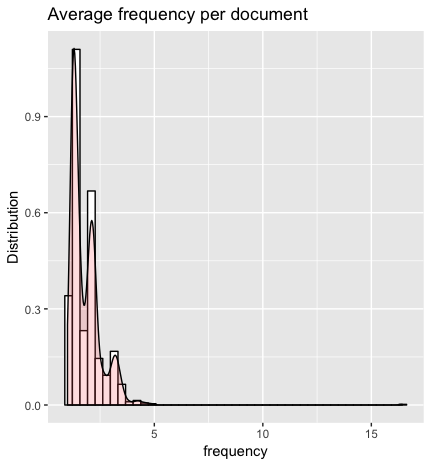
\includegraphics[width=0.9\textwidth]{avgFreq.png}
		\caption{Distribution of the average frequency of tokens per document.}
		\label{fig:1}
		%	\end{minipage}\hfill
		%	\begin{minipage}{0.45\textwidth}
		%		\centering
		%		\includegraphics[width=0.9\textwidth]{frontier-manager.png}
		%		\caption{v2.0 of the worker with a \textit{Frontier Manager} which delegates the workload.}
		%		\label{fig:2}
		%	\end{minipage}
	\end{figure}
	
	\begin{table}[hbt!]
		%	\begin{minipage}{0.45\textwidth}
		\centering
		\begin{tabular}{r|c|c|c}
			Page  &  \#Tokens  &  \#Occurrences  &  Mean  \#Occurrences\\
			\hline
			% word frequency:
			podatki.gov.si.340 & 6528 & 27421 & 4.201 \\
			e-prostor.gov.si.57 & 1679 & 3591 & 2.139 \\
			evem.gov.si.398 & 1559 & 4252 & 2.727 \\
			evem.gov.si.651 & 1292 & 2598 & 2.011 \\
			e-uprava.gov.si.56 & 1191 & 2293 & 1.925 \\
		\end{tabular}
		\caption{Documents with most words}
		\label{tab:6}
		%	\end{minipage}
	\end{table}
	
	\begin{table}[hbt!]
		%	\begin{minipage}{0.45\textwidth}
		\centering
		\begin{tabular}{r|c|c|c}
			% most common word
			Word  &  Frequency  &  Weighted Mean Frequency \footnote{See Section~\ref{sec:analysis} for more details}  &  \#Occurrences \footnote{*\#Occurrences denotes in how many documents the word appears.} \\
			\hline
			podatkov & 11000  &  7.768  &  863 \\
			slovenije & 8814 & 6.225 & 896 \\
			republike & 8356 & 5.901 & 1165 \\
			podatki & 4931 & 3.482 & 732 \\
			navigation & 4474 & 3.160 & 561 \\
		\end{tabular}
		\caption{Basic statistics of the words from the corpus. }
		\label{tab:7}
		%	\end{minipage}
	\end{table}
	
	\section{Conclusion}
	Throughout the paper we introduced our implementation of building inverted index and query against it. Key differences between naive approach of sequential file reading and inverted index are noted supporting with experiments and results which prove how much more efficient the inverted index approach is, which is the reason why that concept is widely used nowadays even though Inverted Index takes much more time in constructing the structure as it allows very efficient querying.
	
	
\end{document}
